\hypertarget{gemoda-s_8c}{
\section{gemoda-s.c File Reference}
\label{gemoda-s_8c}\index{gemoda-s.c@{gemoda-s.c}}
}
{\tt \#include \char`\"{}bit\-Set.h\char`\"{}}\par
{\tt \#include \char`\"{}spat.h\char`\"{}}\par
{\tt \#include \char`\"{}convll.h\char`\"{}}\par
{\tt \#include \char`\"{}matdata.h\char`\"{}}\par
{\tt \#include \char`\"{}Fasta\-Seq\-IO/fasta\-Seq\-IO.h\char`\"{}}\par
{\tt \#include $<$unistd.h$>$}\par
{\tt \#include $<$stdlib.h$>$}\par
{\tt \#include $<$errno.h$>$}\par
{\tt \#include $<$string.h$>$}\par
{\tt \#include \char`\"{}pat\-Stats.h\char`\"{}}\par


Include dependency graph for gemoda-s.c:\begin{figure}[H]
\begin{center}
\leavevmode
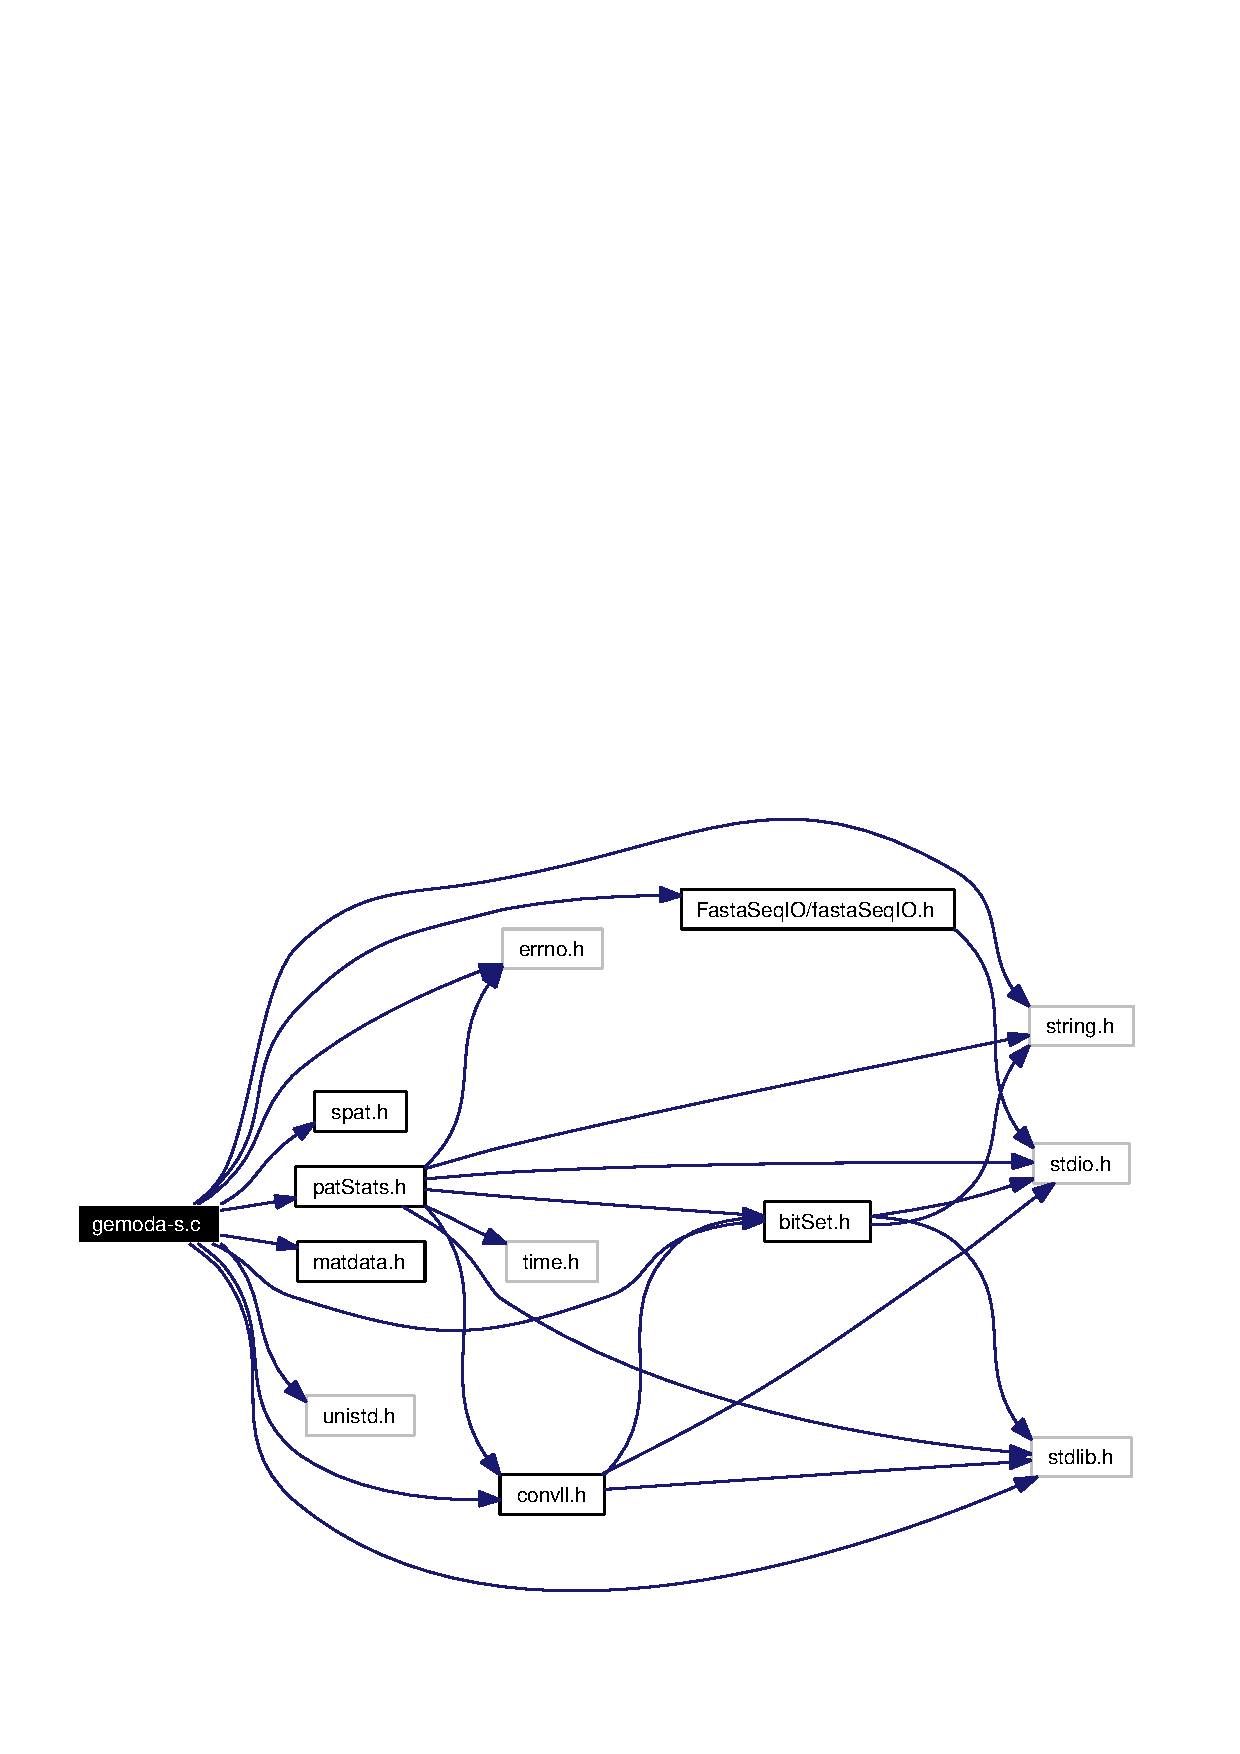
\includegraphics[width=272pt]{gemoda-s_8c__incl}
\end{center}
\end{figure}
\subsection*{Functions}
\begin{CompactItemize}
\item 
void \hyperlink{gemoda-s_8c_a0}{usage} (char $\ast$$\ast$argv)
\item 
void \hyperlink{gemoda-s_8c_a1}{matrixlist} (void)
\item 
void \hyperlink{gemoda-s_8c_a2}{get\-Matrix\-By\-Name} (char \hyperlink{matrixmap_8h_a0}{name}\mbox{[}$\,$\mbox{]}, int \hyperlink{matrixmap_8h_a1}{mat}\mbox{[}$\,$\mbox{]}\mbox{[}MATRIX\_\-SIZE\mbox{]})
\item 
\hyperlink{structbitGraph__t}{bit\-Graph\_\-t} $\ast$ \hyperlink{gemoda-s_8c_a3}{align\-Words\-Mat\_\-bit} (\hyperlink{structsPat__t}{s\-Pat\_\-t} $\ast$words, int wc, int \hyperlink{matrixmap_8h_a1}{mat}\mbox{[}$\,$\mbox{]}\mbox{[}MATRIX\_\-SIZE\mbox{]}, int threshold)
\item 
\hyperlink{structsPat__t}{s\-Pat\_\-t} $\ast$ \hyperlink{gemoda-s_8c_a4}{count\-Words2} (\hyperlink{structfSeq__t}{f\-Seq\_\-t} $\ast$seq, int num\-Seq, int L, int $\ast$num\-Words)
\item 
\hyperlink{structcnode}{cll\_\-t} $\ast$ \hyperlink{gemoda-s_8c_a5}{convolve} (\hyperlink{structbitGraph__t}{bit\-Graph\_\-t} $\ast$bg, int support, int R, int $\ast$index\-To\-Seq, int p, int cluster\-Method, int $\ast$$\ast$offset\-To\-Index, int number\-Of\-Sequences, int no\-Convolve, FILE $\ast$OUTPUT\_\-FILE)
\item 
\hyperlink{structbitGraph__t}{bit\-Graph\_\-t} $\ast$ \hyperlink{gemoda-s_8c_a6}{prune\-Bit\-Graph} (\hyperlink{structbitGraph__t}{bit\-Graph\_\-t} $\ast$bg, int $\ast$index\-To\-Seq, int $\ast$$\ast$offset\-To\-Index, int num\-Of\-Seqs, int p)
\item 
int \hyperlink{gemoda-s_8c_a7}{main} (int argc, char $\ast$$\ast$argv)
\end{CompactItemize}


\subsection*{Detailed Description}
This file houses the main routine for the sequence based Gemoda algorithm. In addition, there are a few helper functions which are used to inform the user how to run the software.

The Gemoda algorithm has three stages: comparison, clustering, and convolution. These three stages are called in serial from the main routine in this file.

Definition in file \hyperlink{gemoda-s_8c-source}{gemoda-s.c}.

\subsection*{Function Documentation}
\hypertarget{gemoda-s_8c_a3}{
\index{gemoda-s.c@{gemoda-s.c}!alignWordsMat_bit@{alignWordsMat\_\-bit}}
\index{alignWordsMat_bit@{alignWordsMat\_\-bit}!gemoda-s.c@{gemoda-s.c}}
\subsubsection[alignWordsMat\_\-bit]{\setlength{\rightskip}{0pt plus 5cm}\hyperlink{structbitGraph__t}{bit\-Graph\_\-t}$\ast$ align\-Words\-Mat\_\-bit (\hyperlink{structsPat__t}{s\-Pat\_\-t} $\ast$ {\em words}, int {\em wc}, int {\em mat}\mbox{[}$\,$\mbox{]}\mbox{[}MATRIX\_\-SIZE\mbox{]}, int {\em threshold})}}
\label{gemoda-s_8c_a3}


This uses the function above. Here, we have an array of words (\hyperlink{structsPat__t}{s\-Pat\_\-t} objects) and we compare (align) them all. If their score is above 'threshold' then we will set a bit to 'true' in a \hyperlink{structbitGraph__t}{bit\-Graph\_\-t} that we create. A \hyperlink{structbitGraph__t}{bit\-Graph\_\-t} is essentially an adjacency matrix, where each member of the matrix contains only a single bit: are the words equal, true or false? The function traverses the words by doing and all by all comparison; however, we only do the upper diagonal. The function makes use of align\-Mat and needs to be passed a scoring matrix that the user has chosen which is appropriate for the context of whatever data sent the user is looking at.

Definition at line 88 of file align.c.

References align\-Mat(), bit\-Graph\-Set\-True\-Sym(), mat, and new\-Bit\-Graph().

Referenced by main().

\scriptsize\begin{verbatim}90 {
91   bitGraph_t * sg = NULL;
92   int score;
93   int i, j;
94   
95     // Assign a new bitGraph_t object, with (wc x wc) possible
96     // true/false values
97     sg = newBitGraph (wc);
98   for (i = 0; i < wc; i++)
99     {
100       for (j = i; j < wc; j++)
101     {
102       
103         // Get the score for the alignment of word i and word j
104         score =
105         alignMat (words[i].string, words[j].string, words[i].length, mat);
106       
107         // If that score is greater than threshold, set
108         // a bit to 'true' in our bitGraph_t object
109         if (score >= threshold)
110         {
111           
112         // We use 'bitGraphSetTrueSym' because, if i=j,
113         // then j=i for most applications.  However, this
114         // can be relaxed for masochists.
115         bitGraphSetTrueSym (sg, i, j);
116         }
117     }
118     }
119   
120     // Return a pointer to this new bitGraph_t object
121     return sg;
122 }
\end{verbatim}
\normalsize 


\hypertarget{gemoda-s_8c_a5}{
\index{gemoda-s.c@{gemoda-s.c}!convolve@{convolve}}
\index{convolve@{convolve}!gemoda-s.c@{gemoda-s.c}}
\subsubsection[convolve]{\setlength{\rightskip}{0pt plus 5cm}\hyperlink{structcnode}{cll\_\-t}$\ast$ convolve (\hyperlink{structbitGraph__t}{bit\-Graph\_\-t} $\ast$ {\em bg}, int {\em support}, int {\em R}, int $\ast$ {\em index\-To\-Seq}, int {\em p}, int {\em cluster\-Method}, int $\ast$$\ast$ {\em offset\-To\-Index}, int {\em number\-Of\-Sequences}, int {\em no\-Convolve}, FILE $\ast$ {\em OUTPUT\_\-FILE})}}
\label{gemoda-s_8c_a5}


Our outer convolution function. This function will call preliminary functions, cluster the data, and then call the main convolution function. This is the interface between the main gemoda-$<$x$>$ code and the generic code that gets all of the work done. Input: the bit\-Graph to be clustered and convolved, the minimum support necessary for a motif to be returned, a flag indicating whether recursive filtering should be used, a pointer to the data structure that dereferences offset indices to sequence numbers, the number of unique source sequences that a motif must be present in, and a number indicating the clustering method that is to be used. Output: the final motif linked list with all motifs that are to be given as output to the user.

Definition at line 625 of file new\-Conv.c.

References bit\-Graph\-Set\-False\-Diagonal(), complete\-Conv(), delete\-Bit\-Set(), fill\-Set(), filter\-Graph(), find\-Cliques(), new\-Bit\-Set(), prune\-Bit\-Graph(), prune\-Cll(), single\-Linkage(), bit\-Graph\_\-t::size, and yank\-Cll().

\scriptsize\begin{verbatim}629 {
630   bitSet_t * cand = NULL;
631   bitSet_t * mask = NULL;
632   bitSet_t * Q = NULL;
633   int size = bg->size;
634   cll_t * elemPats = NULL;
635   cll_t * allCliques = NULL;
636   cll_t * curr = NULL;
637   
638     // contains indices (rows) containing the threshold value.
639     cand = newBitSet (size);
640   mask = newBitSet (size);
641   Q = newBitSet (size);
642   fillSet (cand);
643   fillSet (mask);
644   
645     // Note that we prune based on p before setting the diagonal false.
646     if (p > 1)
647     {
648       bg =
649     pruneBitGraph (bg, indexToSeq, offsetToIndex, numberOfSequences, p);
650     }
651   
652     // Now we set the main diagonal false for clustering and filtering.
653     bitGraphSetFalseDiagonal (bg);
654   filterGraph (bg, support, R);
655   fprintf (OUTPUT_FILE, "Graph filtered!  Now clustering...\n");
656   fflush (NULL);
657   if (clusterMethod == 0)
658     {
659       findCliques (Q, cand, mask, bg, support, 0, &elemPats, indexToSeq, p);
660     }
661   else
662     {
663       singleLinkage (Q, cand, mask, bg, support, 0, &elemPats, indexToSeq,
664               p);
665     }
666   fprintf (OUTPUT_FILE,
667         "Clusters found!  Now filtering clusters (if option set)...\n");
668   fflush (NULL);
669   if (p > 1)
670     {
671       elemPats = pruneCll (elemPats, indexToSeq, p);
672     }
673   deleteBitSet (cand);
674   deleteBitSet (mask);
675   deleteBitSet (Q);
676   
677     // Now let's convolve what we made.
678     if (noConvolve == 0)
679     {
680       fprintf (OUTPUT_FILE, "Now convolving...\n");
681       fflush (NULL);
682       allCliques = completeConv (&elemPats, support, size, 0, indexToSeq, p);
683     }
684   
685   else
686     {
687       curr = elemPats;
688       while (curr != NULL)
689     {
690       yankCll (&elemPats, NULL, &curr, &allCliques, 0);
691     }
692     }
693   return allCliques;
694 }
\end{verbatim}
\normalsize 


\hypertarget{gemoda-s_8c_a4}{
\index{gemoda-s.c@{gemoda-s.c}!countWords2@{countWords2}}
\index{countWords2@{countWords2}!gemoda-s.c@{gemoda-s.c}}
\subsubsection[countWords2]{\setlength{\rightskip}{0pt plus 5cm}\hyperlink{structsPat__t}{s\-Pat\_\-t}$\ast$ count\-Words2 (\hyperlink{structfSeq__t}{f\-Seq\_\-t} $\ast$ {\em seq}, int {\em num\-Seq}, int {\em L}, int $\ast$ {\em num\-Words})}}
\label{gemoda-s_8c_a4}


Counts words of size {\em L\/} in the input Fast\-A sequences, hashes all of the words, and returns an array of \hyperlink{structsPat__t}{s\-Pat\_\-t} objects.

Definition at line 373 of file words.c.

References s\-Hash\-Entry\_\-t::data, destroy\-SHash(), s\-Hash\-Entry\_\-t::idx, init\-SHash(), s\-Hash\-Entry\_\-t::key, s\-Hash\-Entry\_\-t::L, s\-Pat\_\-t::length, s\-Offset\_\-t::next, s\-Pat\_\-t::offset, s\-Offset\_\-t::pos, s\-Offset\_\-t::prev, search\-SHash(), s\-Offset\_\-t::seq, sieve3(), s\-Pat\_\-t::string, and s\-Pat\_\-t::support.

Referenced by main().

\scriptsize\begin{verbatim}374 {
375   int i, j;
376   int totalChars = 0;
377   int hashSize;
378   sHashEntry_t newEntry;
379   sHashEntry_t *ep;
380   sHash_t wordHash;
381   sPat_t *words = NULL;
382   int wc = 0;
383   int prev = -1;
384   int l;
385 
386 
387   // Count the total number of characters.  This
388   // is the upper limit on how many words we can have
389   for (i = 0; i < numSeq; i++)
390     {
391       totalChars += strlen (seq[i].seq);
392     }
393 
394   // Get a prime number for the size of the hash table
395   hashSize = sieve3 ((long) (2 * totalChars));
396   wordHash = initSHash (hashSize);
397 
398   // Chop up each sequence and hash out the words of size L
399   for (i = 0; i < numSeq; i++)
400     {
401       prev = -1;
402 
403       // skip sequences that are too short to have
404       // a pattern
405       if (strlen (seq[i].seq) < L)
406     {
407       continue;
408     }
409       for (j = 0; j < strlen (seq[i].seq) - L + 1; j++)
410     {
411 
412       // Make a hash table entry for this word
413       newEntry.key = &(seq[i].seq[j]);
414       newEntry.data = 1;
415       newEntry.idx = wc;
416       newEntry.L = L;
417 
418       // Check to see if it's already in the hash table
419       ep = searchSHash (&newEntry, &wordHash, 0);
420       if (ep == NULL)
421         {
422 
423           // If it's not, create an entry for it
424           ep = searchSHash (&newEntry, &wordHash, 1);
425 
426           // Increase the size of our word array
427           words = (sPat_t *) realloc (words, (wc + 1) * sizeof (sPat_t));
428           if (words == NULL)
429         {
430           fprintf (stderr, "Error!\n");
431           fflush (stderr);
432         }
433           // Add the new word
434           words[wc].string = &(seq[i].seq[j]);
435           words[wc].length = L;
436           words[wc].support = 1;
437           words[wc].offset =
438         (sOffset_t *) malloc (1 * sizeof (sOffset_t));
439           if (words[wc].offset == NULL)
440         {
441           fprintf (stderr, "\nMemory Error\n%s\n", strerror (errno));
442           fflush (stderr);
443           exit (0);
444         }
445           words[wc].offset[0].seq = i;
446           words[wc].offset[0].pos = j;
447           words[wc].offset[0].prev = prev;
448           words[wc].offset[0].next = -1;
449 
450           if (prev != -1)
451         {
452           words[prev].offset[words[prev].support - 1].next = wc;
453         }
454           prev = wc;
455           wc++;
456 
457         }
458       else
459         {
460 
461           // If it is, increase the count for this word
462           ep->data++;
463 
464           // add a new offset to the word array
465           l = words[ep->idx].support;
466           words[ep->idx].offset =
467         (sOffset_t *) realloc (words[ep->idx].offset,
468                        (l + 1) * sizeof (sOffset_t));
469           words[ep->idx].offset[l].seq = i;
470           words[ep->idx].offset[l].pos = j;
471           words[ep->idx].offset[l].prev = prev;
472           words[ep->idx].offset[l].next = -1;
473 
474           // Update the next/prev
475           if (prev != -1)
476         {
477           words[prev].offset[words[prev].support - 1].next = ep->idx;
478         }
479           prev = ep->idx;
480 
481           // Have to put this down here for cases when we create
482           // a word and it is immeadiately followed by itself!!
483           words[ep->idx].support += 1;
484         }
485     }
486     }
487 
488 
489   destroySHash (&wordHash);
490   *numWords = wc;
491   return words;
492 }
\end{verbatim}
\normalsize 


\hypertarget{gemoda-s_8c_a2}{
\index{gemoda-s.c@{gemoda-s.c}!getMatrixByName@{getMatrixByName}}
\index{getMatrixByName@{getMatrixByName}!gemoda-s.c@{gemoda-s.c}}
\subsubsection[getMatrixByName]{\setlength{\rightskip}{0pt plus 5cm}void get\-Matrix\-By\-Name (char {\em name}\mbox{[}$\,$\mbox{]}, int {\em mat}\mbox{[}$\,$\mbox{]}\mbox{[}MATRIX\_\-SIZE\mbox{]})}}
\label{gemoda-s_8c_a2}




Referenced by main().\hypertarget{gemoda-s_8c_a7}{
\index{gemoda-s.c@{gemoda-s.c}!main@{main}}
\index{main@{main}!gemoda-s.c@{gemoda-s.c}}
\subsubsection[main]{\setlength{\rightskip}{0pt plus 5cm}int main (int {\em argc}, char $\ast$$\ast$ {\em argv})}}
\label{gemoda-s_8c_a7}


This is the main routine of the Gemoda source code. The routine performs basic operations such as parsing the input from the user and opening input files. Then, the function hashes words of length L. The unique words are aligned against each other to produce an adjacency matrix that says whether the unique word i is sufficiently similar, based on the user supplied threshold, to the unique word j. This adjacency matrix is then dereferenced into an adjacency matrix in which each index of the matrix represents a unique position in the input sequences, rather than a unique word. This dereferencing is required for the convolution stage. Finally, this adjacency matrix is convolved and the final motifs are returned as a linked list. The routine then closes all input and output files and frees up dynamically allocated memory.

Definition at line 187 of file gemoda-s.c.

References align\-Words\-Mat\_\-bit(), bit\-Graph\-Check\-Bit(), bit\-Graph\-Set\-True\-Sym(), calc\-Stat\-All\-Cliqs(), convolve(), count\-Words2(), cum\-DMatrix(), delete\-Bit\-Graph(), Free\-FSeqs(), get\-Matrix\-By\-Name(), get\-Stat\-Mat(), cnode::length, mat, MATRIX\_\-SIZE, matrixlist(), c\-Set\_\-t::members, new\-Bit\-Graph(), cnode::next, s\-Pat\_\-t::offset, pop\-All\-Cll(), s\-Offset\_\-t::pos, Read\-FSeqs(), s\-Offset\_\-t::seq, cnode::set, c\-Set\_\-t::size, bit\-Graph\_\-t::size, sort\-By\-Stats(), cnode::stat, and usage().

\scriptsize\begin{verbatim}188 {
189   int inputOption = 0;
190   char *sequenceFile = NULL;
191   char *outputFile = NULL;
192   char *matName = NULL;
193   FILE * SEQUENCE_FILE = NULL;
194   FILE * OUTPUT_FILE = NULL;
195   int L = 0;
196   int numberOfSequences = 0;
197   fSeq_t * mySequences = NULL;
198   fSeq_t * (*seqReadFunct) () = &ReadFSeqs;
199   sPat_t * words = NULL;
200   int wc;
201   int status = 0;
202   int g = 0;
203   int sup = 2;
204   int R = 1;
205   int P = 0;
206   int (*mat)[MATRIX_SIZE] = NULL;
207   int noConvolve = 0;
208   int j, k, i, l;
209   bitGraph_t * bg = NULL;
210   bitGraph_t * oam = NULL;
211   
212     // new
213   int **offsetToIndex = NULL;
214   int *indexToSeq = NULL;
215   int *indexToPos = NULL;
216   int numberOfOffsets = 0;
217   int pos1, pos2;
218   
219     // int *prevRowArray;
220     sOffset_t * offset1, *offset2;
221   cll_t * allCliques = NULL;
222   cll_t * curCliq = NULL;
223   int curSeq;
224   int curPos;
225   int clusterMethod = 0;
226   
227     // patStats
228   int samp = 1;
229   unsigned int **d = NULL;
230   int supportDim = 0, lengthDim = 0;
231   int oamSize = 0;
232   
233     /*
234         Get command-line options  
235      */ 
236     while ((inputOption = getopt (argc, argv, "i:o:l:g:k:m:p:zc:ns:")) != EOF)
237     {
238       switch (inputOption)
239     {
240       
241         // Input file
242     case 'i':
243       sequenceFile = optarg;
244       seqReadFunct = &ReadFSeqs;
245       break;
246       
247         // Output file
248     case 'o':
249       outputFile =
250         (char *) malloc ((strlen (optarg) + 1) * sizeof (char));
251       if (outputFile == NULL)
252         {
253           fprintf (stderr, "Error allocating memory for options.\n");
254           exit (EXIT_FAILURE);
255         }
256       else
257         {
258           strcpy (outputFile, optarg);
259         }
260       break;
261       
262         // Minimum motif length
263     case 'l':
264       L = atoi (optarg);
265       break;
266       
267         // Minimum motif similarity score
268     case 'g':
269       g = atoi (optarg);
270       status++;
271       break;
272       
273         // Minimum support (number of motif occurrences)
274     case 'k':
275       sup = atoi (optarg);
276       break;
277       
278         // Similarity matrix used to find similarity score
279     case 'm':
280       getMatrixByName (optarg, &mat);
281       matName = (char *) malloc (strlen (optarg) * sizeof (char));
282       if (matName == NULL)
283         {
284           fprintf (stderr, "Error allocating memory for options.\n");
285           exit (EXIT_FAILURE);
286         }
287       else
288         {
289           strcpy (matName, optarg);
290         }
291       break;
292       
293 /***************************************************************
294  * Recursive initial pruning: an option for clique finding.
295  *   It takes all nodes with less than the minimum
296  *   number of support and removes all of their nodes, and does this 
297  *   recursively so that nodes that are connected to many sparsely connected
298  *   nodes will be removed and not left in the 
299  * This option is deprecated as it is at worst no-gain and at best useful.
300  *   It will be on by default for clique-finding, but can be turned 
301  *   back off with some
302  *   minor tweaking.  For almost all cases in which it does not speed
303  *   up computations, it will have a trivial time to perform.  Thus, if 
304  *   clique-finding is turned on, then R is set to 1 by default.
305         case 'r':
306             R = 1;
307             break;
308 ************************************************************************/ 
309         // Optional pruning parameter to require at motif occurrences
310         // in at least P distinct input sequences
311     case 'p':
312       P = atoi (optarg);
313       break;
314       
315         // Clustering method.
316     case 'c':
317       clusterMethod = atoi (optarg);
318       break;
319     case 'n':
320       noConvolve = 1;
321       break;
322     case 's':
323       samp = atoi (optarg);
324       break;
325       
326         // Catch-all.
327     case '?':
328       fprintf (stderr, "Unknown option `-%c'.\n", optopt);
329       usage (argv);
330       return EXIT_SUCCESS;
331     case 'z':
332       matrixlist ();
333       return EXIT_SUCCESS;
334     default:
335       usage (argv);
336       return EXIT_SUCCESS;
337     }
338     }
339   
340     // Require a similarity matrix
341     if (mat == NULL)
342     {
343       usage (argv);
344       return EXIT_SUCCESS;
345     }
346   
347     // Require an input file, a nonzero length, and a similarity threshold
348     // to be set.
349     if (sequenceFile == NULL || L == 0 || status < 1)
350     {
351       usage (argv);
352       return EXIT_SUCCESS;
353     }
354   
355     // Open the sequence file
356     if ((SEQUENCE_FILE = fopen (sequenceFile, "r")) == NULL)
357     {
358       fprintf (stderr, "Couldn't open file %s; %s\n", sequenceFile,
359         strerror (errno));
360       exit (EXIT_FAILURE);
361     }
362   
363     // Open the output file
364     if (outputFile != NULL)
365     {
366       if ((OUTPUT_FILE = fopen (outputFile, "w")) == NULL)
367     {
368       fprintf (stderr, "Couldn't open file %s; %s\n", outputFile,
369             strerror (errno));
370       exit (EXIT_FAILURE);
371     }
372     }
373   else
374     {
375       OUTPUT_FILE = stdout;
376     }
377   
378     // Allocate some sequences
379     mySequences = seqReadFunct (SEQUENCE_FILE, &numberOfSequences);
380   if (mySequences == NULL)
381     {
382       fprintf (stderr, "\nError reading your sequences/text.");
383       fprintf (stderr, "\nCheck the format/size of the file.");
384       fprintf (stderr, "\nERROR:  %s\n", strerror (errno));
385       return EXIT_FAILURE;
386     }
387   
388     // Close the input files
389     fclose (SEQUENCE_FILE);
390   
391     // Verbosity in output helps to distinguish output files.
392     fprintf (OUTPUT_FILE, "\nMatrix used = %s\n", matName);
393   fprintf (OUTPUT_FILE, "Input file = %s\n", sequenceFile);
394   fprintf (OUTPUT_FILE, "l = %d, k = %d, g = %d\n", L, sup, g);
395   if (P > 1)
396     {
397       fprintf (OUTPUT_FILE, "Minimum # of sequences with motif = %d\n", P);
398     }
399   if (R > 0)
400     {
401       fprintf (OUTPUT_FILE, "Recursive pruning is ON.\n");
402     }
403   
404     // Find the unique words in the input.
405     words = countWords2 (mySequences, numberOfSequences, L, &wc);
406   
407     /*
408        fprintf(stderr, "Counted %d words\n", wc);
409      */ 
410     /*
411        fflush(stderr);
412      */ 
413     
414     // Align the words that we just found by applying the similarity
415     // matrix to each pair of them.  Note that
416     // bg is the adjacency matrix of words, but we
417     // need an adjacency matrix of offsets instead.  
418     bg = alignWordsMat_bit (words, wc, mat, g);
419   fprintf (OUTPUT_FILE, "\nAligned!  Creating offset matrix...\n");
420   fflush (NULL);
421   
422     // Create an intermediate translation matrix
423     // to store the offset number of each sequence number/position.
424     // 
425     // Note that this matrix is better called "Index to offset", and
426     // the other matrices are better called "offset to Seq" and
427     // "offset to Pos"
428     offsetToIndex = (int **) malloc (numberOfSequences * sizeof (int *));
429   if (offsetToIndex == NULL)
430     {
431       fprintf (stderr,
432         "Unable to allocate memory - offsetToIndex in gemoda.c\n%s\n",
433         strerror (errno));
434       fflush (stderr);
435       exit (0);
436     }
437   for (i = 0; i < numberOfSequences; i++)
438     {
439       
440     // MPS 5/23/05: Added in "-L+2" to make there only be one
441     // blank between sequences.
442     offsetToIndex[i] =
443     malloc ((strlen (mySequences[i].seq) - L + 2) * sizeof (int));
444       if (offsetToIndex[i] == NULL)
445     {
446       fprintf (stderr,
447             "Unable to allocate memory - offsetToIndex[%d] in gemoda.c\n%s\n",
448             i, strerror (errno));
449       fflush (stderr);
450       exit (0);
451     }
452       
453     // MPS 5/23/05: Added in "-L+2" to make there only be one
454     // blank between sequences.
455     for (j = 0; j < (strlen (mySequences[i].seq) - L + 2); j++)
456     {
457       offsetToIndex[i][j] = numberOfOffsets;
458       numberOfOffsets++;
459     }
460     }
461   
462     // Now create translation matrices such that we can get the sequence
463     // or position number of a given offset.
464     indexToSeq = (int *) malloc (numberOfOffsets * sizeof (int));
465   if (indexToSeq == NULL)
466     {
467       fprintf (stderr,
468         "Unable to allocate memory - indexToSeq in gemoda.c\n%s\n",
469         strerror (errno));
470       fflush (stderr);
471       exit (0);
472     }
473   indexToPos = (int *) malloc (numberOfOffsets * sizeof (int));
474   if (indexToPos == NULL)
475     {
476       fprintf (stderr,
477         "Unable to allocate memory - indexToPos in gemoda.c\n%s\n",
478         strerror (errno));
479       fflush (stderr);
480       exit (0);
481     }
482   k = 0;
483   for (i = 0; i < numberOfSequences; i++)
484     {
485       
486     // MPS 5/23/05: Added in "-L+2" to make there only be one
487     // blank between sequences.
488     for (j = 0; j < (strlen (mySequences[i].seq) - L + 2); j++)
489     {
490       indexToSeq[k] = i;
491       indexToPos[k] = j;
492       k++;
493     }
494     }
495   
496     // Now make an offset adjacency matrix! 
497     // 
498     oam = newBitGraph (numberOfOffsets);
499   
500     // Go through each unique word
501     for (i = 0; i < wc; i++)
502     {
503       offset1 = words[i].offset;
504       
505     // Go through each occurrence
506     for (k = 0; k < words[i].support; k++)
507     {
508       
509         // Use the offsetToIndex translation to get the offset
510         // of the first occurrence
511         pos1 = offsetToIndex[offset1[k].seq][offset1[k].pos];
512       
513         // And go through each word in the first offset to 
514         // find words that meet the similarity threshold
515         for (j = 0; j < wc; j++)
516         {
517           if (bitGraphCheckBit (bg, i, j))
518         {
519           offset2 = words[j].offset;
520           
521             // And find all of their occurrences,
522             // using offsetToIndex to get the
523             // offsets, and then setting those
524             // locations in the offset adjacency
525             // matrix true.
526             for (l = 0; l < words[j].support; l++)
527             {
528               pos2 = offsetToIndex[offset2[l].seq][offset2[l].pos];
529               bitGraphSetTrueSym (oam, pos1, pos2);
530             }
531         }
532         }
533     }
534     }
535   fprintf (OUTPUT_FILE, "Offset matrix created...");
536   deleteBitGraph (bg);
537   if ((samp > 0) && (clusterMethod == 0))
538     {
539       fprintf (OUTPUT_FILE, " taking preliminary statistics.\n");
540       fflush (NULL);
541       d =
542     getStatMat (oam, sup, L, &supportDim, &lengthDim, numberOfSequences,
543             samp, OUTPUT_FILE);
544       fprintf (OUTPUT_FILE, "Now filtering...\n");
545       fflush (NULL);
546     }
547   else
548     {
549       fprintf (OUTPUT_FILE, " now filtering.\n");
550       fflush (NULL);
551       d = NULL;
552       supportDim = 0;
553     }
554   
555     // Now we're convolving on offsets
556     allCliques =
557     convolve (oam, sup, R, indexToSeq, P, clusterMethod, offsetToIndex,
558           numberOfSequences, noConvolve, OUTPUT_FILE);
559   
560     // Do some early memory cleanup to limit usage
561     oamSize = oam->size;
562   deleteBitGraph (oam);
563   fprintf (OUTPUT_FILE, "Convolved!  Now making output...\n");
564   fflush (NULL);
565   if ((samp > 0) && (clusterMethod == 0))
566     {
567       cumDMatrix (d, allCliques, supportDim, lengthDim, oamSize,
568            numberOfSequences);
569       calcStatAllCliqs (d, allCliques, numberOfOffsets - numberOfSequences);
570       allCliques = sortByStats (allCliques);
571     }
572   
573     // walk over the cliques and give some output in the format:
574     // pattern <pattern id num>: len=<motif length> sup=<motif instances>
575     // <sequence num> <position num> <motif instance>
576     // ...
577     curCliq = allCliques;
578   
579     i = 0;
580   while (curCliq != NULL)
581     {
582       fprintf (OUTPUT_FILE, "pattern %d:\tlen=%d\tsup=%d", i,
583         curCliq->length + L, curCliq->set->size);
584       if (d != NULL)
585     {
586       fprintf (OUTPUT_FILE, "\tsignif=%le\n", curCliq->stat);
587     }
588       else
589     {
590       fprintf (OUTPUT_FILE, "\n");
591     }
592       
593     for (j = 0; j < curCliq->set->size; j++)
594     {
595       pos1 = curCliq->set->members[j];
596       curSeq = indexToSeq[pos1];
597       curPos = indexToPos[pos1];
598       fprintf (OUTPUT_FILE, "   %d\t%d\t", curSeq, curPos);
599       for (k = curPos; k < curPos + curCliq->length + L; k++)
600         {
601           fprintf (OUTPUT_FILE, "%c", mySequences[curSeq].seq[k]);
602         }
603       fprintf (OUTPUT_FILE, "\n");
604     }
605       fprintf (OUTPUT_FILE, "\n\n");
606       curCliq = curCliq->next;
607       i++;
608     }
609   
610     // And do some memory cleanup
611     // And cleanup of probability stuff...
612     /*
613         free(letterfreqs); delete_augmented_matrix(augmat); 
614      */ 
615     allCliques = popAllCll (allCliques);
616   free (indexToSeq);
617   indexToSeq = NULL;
618   free (indexToPos);
619   indexToPos = NULL;
620   for (i = 0; i < numberOfSequences; i++)
621     {
622       free (offsetToIndex[i]);
623       offsetToIndex[i] = NULL;
624     }
625   
626     // Free'ing added by MPS, 6/4
627     for (i = 0; i < wc; i++)
628     {
629       free (words[i].offset);
630     }
631   free (words);
632   
633     // End free'ing added by MPS
634     free (offsetToIndex);
635   offsetToIndex = NULL;
636   
637     // -------------------------------------------
638     
639     // Free up fastaSequences
640     FreeFSeqs (mySequences, numberOfSequences);
641   fclose (OUTPUT_FILE);
642   return 0;
643 }
\end{verbatim}
\normalsize 


\hypertarget{gemoda-s_8c_a1}{
\index{gemoda-s.c@{gemoda-s.c}!matrixlist@{matrixlist}}
\index{matrixlist@{matrixlist}!gemoda-s.c@{gemoda-s.c}}
\subsubsection[matrixlist]{\setlength{\rightskip}{0pt plus 5cm}void matrixlist (void)}}
\label{gemoda-s_8c_a1}


This function prints a list of the matrices that Gemoda can use to do the alignment of words. Most of these matrices are appropriate for amino acid sequences. In addition, there are matrices for DNA sequences and an identity matrix that is appropriate for other sequences, such as the analysis of English text. The matrix is selected using the -m flag.

Definition at line 99 of file gemoda-s.c.

Referenced by main().

\scriptsize\begin{verbatim}100 {
101   fprintf (stdout, "\nThe following similarity matrices are installed " 
102         "with the default Gemoda installation.\n  Most of these " 
103         "were obtained from publically available BLAST distributions. \n\n"
104          "dna_idmat:\n\t" 
105         "Identity matrix for DNA: returns 1 when A,C,G,T are " 
106         "compared to \n\tthemselves, 0 otherwise.\n\n" 
107         "identity_aa:\n\t" 
108         "Identity matrix for amino acids: returns 1 when any \n\t" 
109         "letter but J,O,U are compared to themselves, and 0 " 
110         "otherwise.\n\n"  "idmat:\n\t" 
111         "Similar to identity_aa, but it returns 10 in place " 
112         "of 1.\n\n"  "est_idmat:\n\t" 
113         "Similar to idmat, but it returns -10 in place of 0. "  "\n\n" 
114         "pam100:\n"  "pam110:\n"  "pam120:\n"  "pam130:\n" 
115         "pam140:\n"  "pam150:\n"  "pam160:\n"  "pam190:\n" 
116         "pam200:\n"  "pam210:\n"  "pam220:\n"  "pam230:\n" 
117         "pam240:\n"  "pam250:\n"  "pam260:\n"  "pam280:\n" 
118         "pam290:\n"  "pam300:\n"  "pam310:\n"  "pam320:\n" 
119         "pam330:\n"  "pam340:\n"  "pam360:\n"  "pam370:\n" 
120         "pam380:\n"  "pam390:\n"  "pam400:\n"  "pam430:\n" 
121         "pam440:\n"  "pam450:\n"  "pam460:\n"  "pam490:\n" 
122         "pam500:\n\t" 
123         "PAM matrices for various evolutionary distances.\n\n" 
124         "blosum30:\n"  "blosum35:\n"  "blosum40:\n"  "blosum45:\n" 
125         "blosum50:\n"  "blosum55:\n"  "blosum60:\n"  "blosum62:\n" 
126         "blosum65:\n"  "blosum70:\n"  "blosum75:\n"  "blosum80:\n" 
127         "blosum85:\n"  "blosum90:\n"  "blosum100:\n\t" 
128         "BLOSUM matrices for various evolutionary distances.\n\n" 
129         "blosumn:\n\t"  "BLOSUM matrix of unknown origin.\n\n" 
130         "dayhoff:\n\t" 
131         "'Vanilla-flavored' pam250, very similar to pam250.\n\n" 
132         "phat_t75_b73:\n"  "phat_t80_b78:\n"  "phat_t85_b82:\n\t" 
133         "BLOSUM-clustered scoring matrix with target frequency\n\t" 
134         "PHDhtm clustering = {75,80,85}percent and background frequency\n\t"
135          "Persson-Argos clustering = {73,78,82}percent.\n\t" 
136         "From Ng, Henikoff, & Henikoff, Bioinformatics 16: 760.\n\n" 
137         "coil_mat:\n"  "alpha_mat:\n"  "beta_mat:\n\t" 
138         "Three structure-specific matrices described by Luthy,\n\t" 
139         "McLachlan, and Eisenberg in Proteins 10, 229-239, obtained from AAindex.\n\n");
140   fprintf (stdout, "\n");
141 } 
\end{verbatim}
\normalsize 


\hypertarget{gemoda-s_8c_a6}{
\index{gemoda-s.c@{gemoda-s.c}!pruneBitGraph@{pruneBitGraph}}
\index{pruneBitGraph@{pruneBitGraph}!gemoda-s.c@{gemoda-s.c}}
\subsubsection[pruneBitGraph]{\setlength{\rightskip}{0pt plus 5cm}\hyperlink{structbitGraph__t}{bit\-Graph\_\-t}$\ast$ prune\-Bit\-Graph (\hyperlink{structbitGraph__t}{bit\-Graph\_\-t} $\ast$ {\em bg}, int $\ast$ {\em index\-To\-Seq}, int $\ast$$\ast$ {\em offset\-To\-Index}, int {\em num\-Of\-Seqs}, int {\em p})}}
\label{gemoda-s_8c_a6}


Simple function (non-recursive) to prune off the first level of motifs that will not meet the \char`\"{}minimum number of unique sequences\char`\"{} criterion. This could have been implemented as above, but it may have gotten a little expensive with less yield, so only the first run through is done here. Input: a bit graph to be pruned, a pointer to the structure that dereferences offset indices to sequence numbers, a pointer to the structure that dereferences seq/position to offsets, the number of unique sequences in the input set, and the minimum number of unique sequences that must contain the motif. Output: a pruned bit\-Graph.

Definition at line 402 of file new\-Conv.c.

References empty\-Set(), bit\-Graph\_\-t::graph, and next\-Bit\-Bit\-Set().

\scriptsize\begin{verbatim}404 {
405   int i = 0, j = 0, nextBit = 0;
406   int *seqNums = NULL;
407   
408     // Since we don't immediately know which node is in which source 
409     // sequence, we can't just count them up regularly.  Instead, we'll
410     // need to keep track of which sequences they come from and 
411     // increment _something_.  What we chose to do here is just make
412     // an array of integers of length = <p>.  Then, we try to put the
413     // source sequence number of each neighbor (including itself, since
414     // the main diagonal is still true at this time) into the next slot
415     // Since we will monotonically search the bitSet, we can just 
416     // move on to the first bit in the next sequence using the 
417     // offsetToIndex structure so that we know the next sequence number
418     // to be put in is always unique.
419     seqNums = (int *) malloc (p * sizeof (int));
420   if (seqNums == NULL)
421     {
422       fprintf (stderr, "Memory error - pruneBitGraph\n%s\n",
423         strerror (errno));
424       fflush (stderr);
425       exit (0);
426     }
427   
428     // So, for each row in the bitgraph...
429     for (i = 0; i < bg->size; i++)
430     {
431       
432     // Make sure the whole array is -1 sentinels.
433     for (j = 0; j < p; j++)
434     {
435       seqNums[j] = -1;
436     }
437       j = 0;
438       
439     // Find the first neighbor of this bit.
440     nextBit = nextBitBitSet (bg->graph[i], 0);
441       if (nextBit == -1)
442     {
443       continue;
444     }
445       else
446     {
447       
448         // and put its sequence number in the array of ints.
449         seqNums[0] = indexToSeq[nextBit];
450     }
451       
452     // If it's the last sequence, then bail out so that we don't
453     // segfault in the next step.
454     if (seqNums[0] >= numOfSeqs - 1)
455     {
456       emptySet (bg->graph[i]);
457       continue;
458     }
459       
460     // Find the next neighbor of this bit, STARTING AT the first
461     // bit in the next sequence.
462     nextBit =
463     nextBitBitSet (bg->graph[i],
464                offsetToIndex[indexToSeq[nextBit] + 1][0]);
465       
466     // And iterate this until we run out of neighbors.
467     while (nextBit >= 0)
468     {
469       j++;
470       seqNums[j] = indexToSeq[nextBit];
471       
472         // Or until this new neighbor will fill up the array
473         if (j == p - 1)
474         {
475           break;
476         }
477       
478         // Or until this new neighbor is in the last sequence.
479         if (seqNums[j] >= numOfSeqs - 1)
480         {
481           break;
482         }
483       
484         // Get the next neighbor!
485         nextBit =
486         nextBitBitSet (bg->graph[i],
487                offsetToIndex[indexToSeq[nextBit] + 1][0]);
488     }
489       
490     // If we didn't have enough unique sequences, and either a) we
491     // were in the nth-to-last sequence and there were no 
492     // neighbors after it, or b) we were in the last sequence,
493     // then the last number will still be our sentinel, -1.  If
494     // the last number is not a sentinel, then we have at least
495     // p distinct sequence occurrences, so we're OK.
496     if (seqNums[p - 1] == -1)
497     {
498       emptySet (bg->graph[i]);
499     }
500     }
501   free (seqNums);
502   return (bg);
503 }
\end{verbatim}
\normalsize 


\hypertarget{gemoda-s_8c_a0}{
\index{gemoda-s.c@{gemoda-s.c}!usage@{usage}}
\index{usage@{usage}!gemoda-s.c@{gemoda-s.c}}
\subsubsection[usage]{\setlength{\rightskip}{0pt plus 5cm}void usage (char $\ast$$\ast$ {\em argv})}}
\label{gemoda-s_8c_a0}


This function describes the basic usage of Gemoda. It is invoked whenever the user submits poor input parameters or selects the help parameter. The function prints a list of possible parameters for Gemoda.

Definition at line 32 of file gemoda-s.c.

\scriptsize\begin{verbatim}33 {
34   fprintf (stdout, "Usage: %s -i <Fasta sequence file> " 
35         "-l <word size> \n\t-k <support> -g <threshold>"
36         "-m <matrix name> [-z] \n\t[-c <cluster method [0|1]>]"
37         "[-p <unique support>] \n\n\n"
38          "Required flags and input:\n\n" 
39         "-i <Fasta sequence file>:\n\t" 
40         "File containing all sequences to be searched, in Fasta format.\n\n"
41          "-l <word size>:\n\t" 
42         "Minimum length of motifs; also the sliding window length\n\t" 
43         "over which all motifs must meet the similarity criterion\n\n" 
44         "-k <support>:\n\t"  "Minimum number of motif occurrences.\n\n" 
45         "-g <threshold>:\n\t" 
46         "Similarity threshold.  Two windows, when scored with the\n\t" 
47         " similarity matrix defined by the -m flag, must have at least\n\t"
48         
49         " this score in order to be deemed 'connected'.  This criterion\n\t"
50          " must be met over all sliding windows of length l.\n\n" 
51         "-m <matrix name>:\n\t" 
52         "Name of the similarity matrix to be used to compare windows.\n\t"
53          "Use -z to see a list of matrices installed by default.\n\n\n" 
54         "Optional flags and input:\n\n"  "-z:\n\t" 
55         "Lists all of the similarity matrices available with the\n\t" 
56         "initial installation of Gemoda.  Note that this overrides\n\t" 
57         "all other options and will only give this output.\n\n" 
58         "-c <cluster method [0|1]>:\n\t" 
59         "The clustering method to be used after evaluating the " 
60         "\n\tsimilarity of the unique words in the input.  Note that the "
61         
62         "\n\tclustering method will have a significant impact on both the "
63          "\n\tresults that one obtains and the computation time.\n\n\t" 
64         "0: clique-finding\n\t\t" 
65         "Uses established methods to find all maximal cliques in the " 
66         "\n\t\tdata.  This will give the most thorough results (that are "
67         
68         "\n\t\tprovably exhaustive), but will also give less-significant "
69          "\n\t\tresults in addition to the most interesting and most\n\t"
70         
71         "significant ones.  The results are deterministic but may take some "
72         
73         "\n\t\ttime on data sets with high similarity or if the similarity "
74          "\n\t\tthreshold is set extremely low.\n\t" 
75         "1: single-linkage clustering\n\t\t" 
76         "Uses a single-linkage-type clustering where all nodes that " 
77         "\n\t\tare connected are put in the same cluster.  This method is "
78         
79         "\n\t\talso deterministic and will be faster than clique-finding, "
80         
81         "\n\t\tbut it loses guarantees of exhaustiveness in searching the "
82          "\n\t\tdata set.\n\n"  "-p <unique support>:\n\t" 
83         "A pruning parameter that requires the motif to occur in " 
84         "\n\tat least <unique support> different input sequences.  Note "
85         
86         "\n\tthat this parameter must be less than or equal to the total "
87          "\n\tsupport parameter set by the -k flag.\n\n", argv[0]);
88   fprintf (stdout, "\n");
89 } 
\end{verbatim}
\normalsize 


